\section{Structure of the source code}

\subsection{Microservices}
Here the code regarding the microservices architecture is explained. \\
The source code that meets the requirements mentioned above has been organized in the following way: for each microservices a project
has been set up. 
Indeed, when dealing with this type of architecture, one should think of a microservice
as a project that should me as much independent as possible from the others: this is the reason that stands behind the choice that has been
made. 
Of course, in this way, it is possible to easily generate the single jars that will be deployed, when necessary, with, as mentioned
in the design document, dockers. Therefore, the following projects are present: API gateway, service registry, group individual request
service, individual request service and share data service. 
As one may notice, the one containing the set up of the API gateway also accesses all the information related with the accounts, and, therefore, authentication and authorization functions are coded here.
In the following sections the structure of the single projects are analyzed. 

\subsubsection{API Gateway}
In the figure ~\ref{fig:pkgapigateway}, it is shown the root of the project structure. An analysis 
of the various elements follows below the figure. 
\begin{figure}[H]
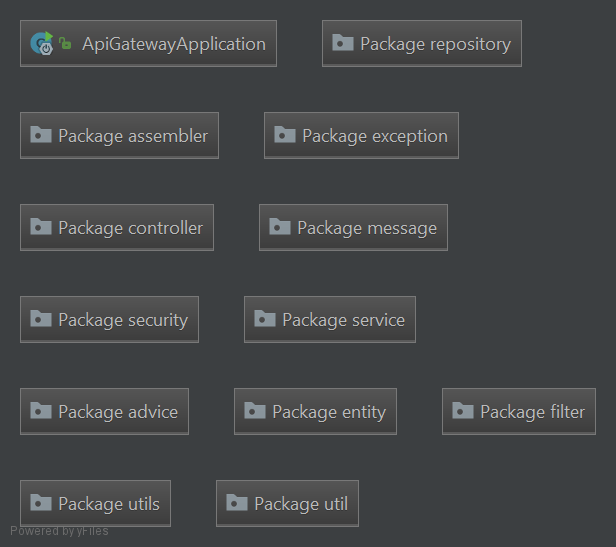
\includegraphics[width=\linewidth]{images/PackageApigateway.png}
\caption{ API gateway }
\label{fig:pkgapigateway}
\end{figure}

\begin{itemize}
\item Package repository: contains the JPA repository for accessing the persistent data necessary to this
service. 
In particular information regarding the accounts of users and third party customers are present. For what concerns the third party customers,
since they can register both as private and as related with a company the following repositories are present: company details, private
details, third party customers and users. An additional repository is present, and it accesses information regarding the API. Indeed, all
the accessible APIs that are available are stored in a database, in order to provide access control. For better specifying this choice, 
one may consider the fact that it is not necessary to search on the service registry non-existing API or to forward requests that can
be already classified as rejected (e.g. user A that is trying to access an API available only for third party customers)
\item Package assembler: this class contains components useful to build HATEOAS resources of entities that are returned to clients, adding
hypermedia contents
\item Package exception: this contains the custom exceptions defined during the development
\item Package controller: contains the controller that defines the APIs that regards the management of the users and third party customer
accounts. From here, it is possible to access the business functions that regards the account (e.g. login, logout, registration). Inside here,
controller are split into secure and public controllers: the public one are accessible to everyone, while for accessing the secured ones,
it is necessary to perform the log in
\item Package message: it provides the functions of communicating with other microservices, by means of RabbitMQ. In particular, three
subpackages are present here. The package publisher contains classes that helps in publishing the events of creation of new accounts to other
other services. The package protocol defines a way of communicating the interested pieces of information, and, finally the configuration
package specifies the configuration settings needed to convert object from JSON (and viceversa) during the exchange of data, and also
the Rabbit queues  
\item Package security: contains the main features that have been introduced above regarding the security 
\item Package service: contains the services that implements the business functions of the account service, with all the APIs that it exposes.
The interfaces present here map the component interfaces of the account service
\item Package advice: this encompasses the handling of server side exceptions in order to show to clients useful messages without exposing
the structure of the project and low level errors
\item Package entity: here classes that are mapped to the databases are present   
\item Package filter: it includes filters that the API gateway applies during the management of "external" requests (i.e. requests that
need to be processed by other services). In particular, it is further subdivided into three packages: pre, route and post. In this case, the
pre filter that is present perform access control on the external API that is being requested, the route filter is a translation filter
that adds header in order to identify the clients in the other microservices, and the post filter fixes the hypermedia content that is sent
as a response to the original request
\item Package util: various utility needed in the development
\end{itemize}

The routes to the other microservices available are present in the application.properties file.

\subsubsection{Service registry}
The project of the service registry is almost empty, no package is present, but just an application class is present, annotated with 
@EnableEurekaServer. The configuration of the service registry is set in the application.properties file.

\subsubsection{Individual request service}
Here it follows the package diagram of the individual request service project ~\ref{fig:pkgindividualrequest}. 
As one may notice, the structure is very similar to the one explained in the api gateway project. 
Of course, here, the controllers provide access to the APIs that regards the individual request service. 
The business functions of this project are present in the  service package, and the interfaces that are present, 
are mapped with the component interfaces of the Design document. \\
Another difference w.r.t. the API gateway that is worth to point out is that here the package message contains also a subpackages that
defines listeners: these are charged of listening to new events that are forwarded from RabbitMQ. 

\begin{figure}[H]
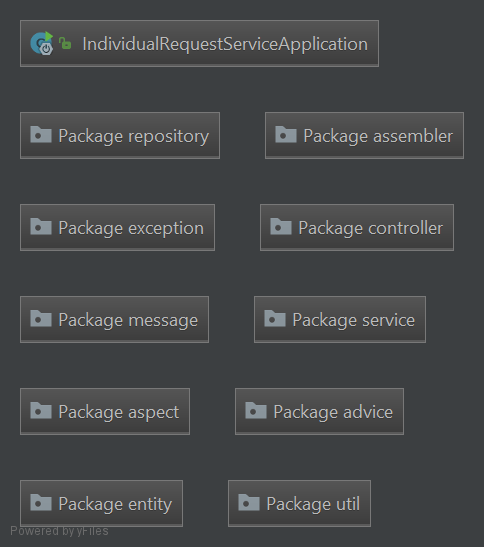
\includegraphics[width=\linewidth]{images/PackageIndividualrequestservice.png}
\caption{ Individual request service }
\label{fig:pkgindividualrequest}
\end{figure}

\subsubsection{Group request service}
In the next figure, the package diagram of the group request project is shown ~\ref{fig:pkggrouprequest}. \\
The same comments hold here except for the fact that the business function mapped in the component interfaces are the one regarding
the group request service. 

\begin{figure}[H]
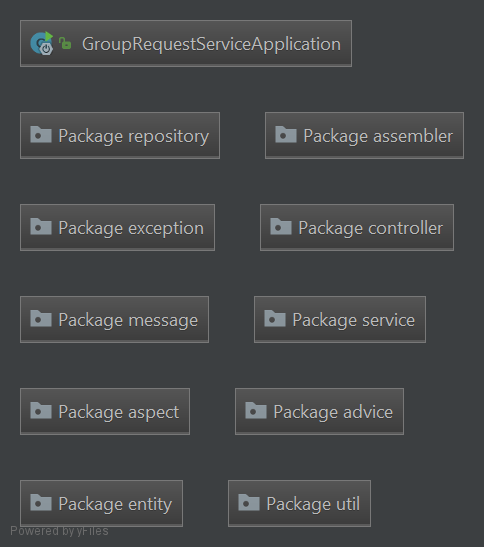
\includegraphics[width=\linewidth]{images/PackageGrouprequestservice.png}
\caption{ Group request service }
\label{fig:pkggrouprequest}
\end{figure}

\subsubsection{Share data service}
The structure of the share data service, as shown by the following picture, is also very similar to the previous ones 
~\ref{fig:pkgsharedata}.

\begin{figure}[H]
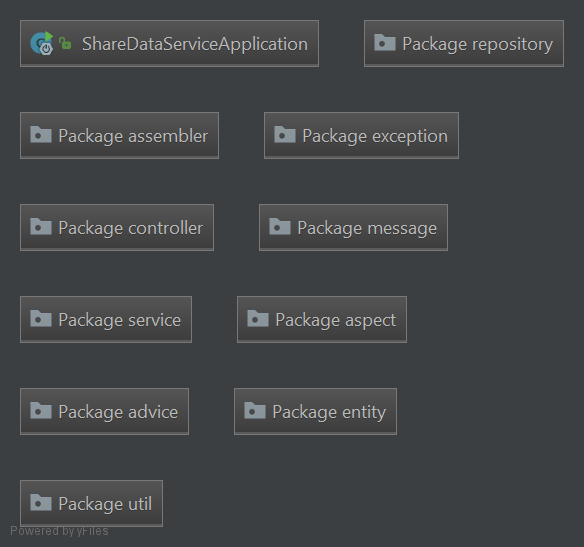
\includegraphics[width=\linewidth]{images/PackageSharedataservice.png}
\caption{ Share data service }
\label{fig:pkgsharedata}
\end{figure}

However, it is important to point out the structure of the code that manages the personalized query specified by the group requests on 
anonymized data. // TODO TANG
  


\subsection{Mobile code}

\subsubsection{Data4Help}
TODO MATTIA

\subsubsection{AutomatedSOS}
TODO TANG TANG

